\documentclass{scrartcl}
\usepackage[layout=a3paper,margin=1in,centering,includefoot]{geometry}
\usepackage{tikz}
\usetikzlibrary{calendar}

% Taking from https://tex.stackexchange.com/a/10199
\makeatletter%
\tikzoption{day headings}{\tikzstyle{day heading}=[#1]}
\tikzstyle{day heading}=[]
\tikzstyle{day letter headings}=[
    execute before day scope={ \ifdate{day of month=1}{%
      \pgfmathsetlength{\pgf@ya}{\tikz@lib@cal@yshift}%
      \pgfmathsetlength\pgf@xa{\tikz@lib@cal@xshift}%
      \pgftransformyshift{-\pgf@ya}
      \foreach \d/\l in {0/M,1/T,2/W,3/T,4/F,5/S,6/S} {
        \pgf@xa=\d\pgf@xa%
        \pgftransformxshift{\pgf@xa}%
        \pgftransformyshift{20pt}%
        \node[every day,day heading]{\l};%
      } 
    }{}%
  }%
]

\makeatother%

\begin{document}
\pagestyle{empty}
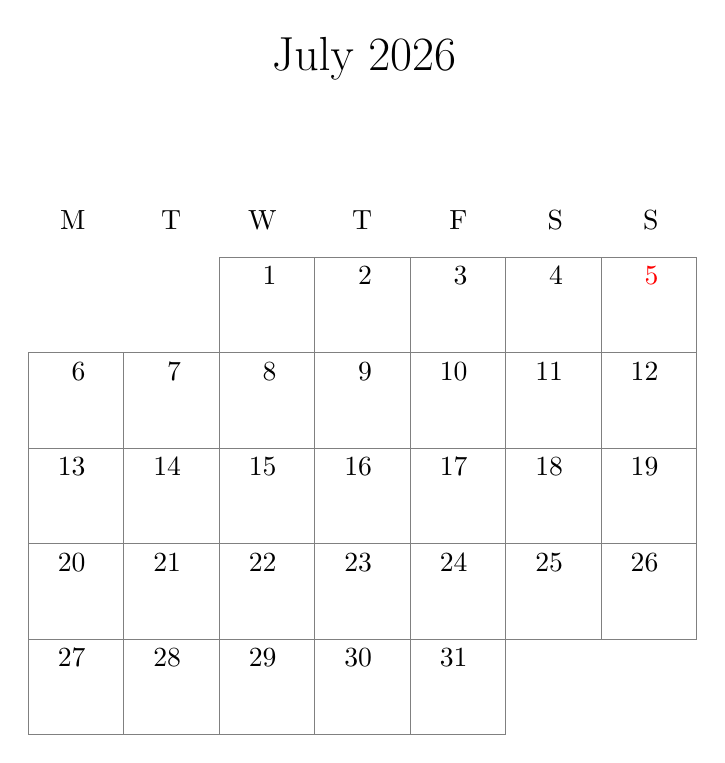
\begin{tikzpicture}
    \calendar [
      name=cal,
        dates=\year-\month-01 to \year-\month-last,
        week list,
        day text=\%d-,
        day xshift=\textwidth/10,
        day yshift=\textwidth/10,
        month label above centered,
        month text={\LARGE {\%mt} \%y-},
        day letter headings
        ]
      if (equals=\year-\month-05) [red]
      if (all) {
      \draw[gray] ++({-\textwidth/20-7pt},10pt) rectangle ++(\textwidth/10,-\textwidth/10);
      };
  \end{tikzpicture}
\end{document}